\subsection{Shining a Light on Narrow-Band Roofing Filters!}

\begin{tcolorbox}[colback=gray!10, colframe=black, title=E4C12] How does a narrow-band roofing filter affect receiver performance?
\begin{enumerate}[label=\Alph*),noitemsep]
    \item It improves sensitivity by reducing front-end noise
    \item It improves intelligibility by using low Q circuitry to reduce ringing
    \item \textbf{It improves blocking dynamic range by attenuating strong signals near the receive frequency}
    \item All these choices are correct
\end{enumerate} \end{tcolorbox}

\subsubsection{Explanation of the Correct Answer}


A narrow-band roofing filter is employed in radio receivers to enhance their performance by selectively filtering out unwanted signals. This is particularly important in environments where multiple signals may be present around the frequency of interest. Narrow-band roofing filters allow signals within a specific frequency range to pass through while attenuating or blocking those that fall outside this range. This selective filtering helps to improve the receiver's blocking dynamic range.

\subsubsection{Related Concepts}
To understand the impact of a narrow-band roofing filter on receiver performance, it is important to be familiar with the following concepts:

1. \textbf{Sensitivity}: This refers to the receiver's ability to discern weak signals from background noise. While a roofing filter can help reduce noise, its primary purpose is not to directly improve sensitivity but to manage out-of-band signals.

2. \textbf{Blocking Dynamic Range}: This is a measure of how well a receiver can handle strong signals without distortion. A good blocking dynamic range indicates that the receiver can remain functional and effective even in the presence of strong signals close to the desired frequency.

3. \textbf{Selectivity}: This is the capability of a receiver to isolate the frequency of interest from adjacent frequencies. The narrow-band roofing filter enhances the selectivity of the receiver, allowing it to better distinguish the desired signal from others.

4. \textbf{Q Factor}: This describes the quality of a resonant circuit. A low Q factor implies a wider bandwidth, which can lead to increased ringing in the response. This is not typically desired when using roofing filters, which often have a high Q factor to ensure they effectively filter signals.

\subsubsection{Calculation and Diagram}
While there are no specific calculations required for this question, we can conceptualize the impact of the roofing filter with a simple diagram. 

\begin{center}
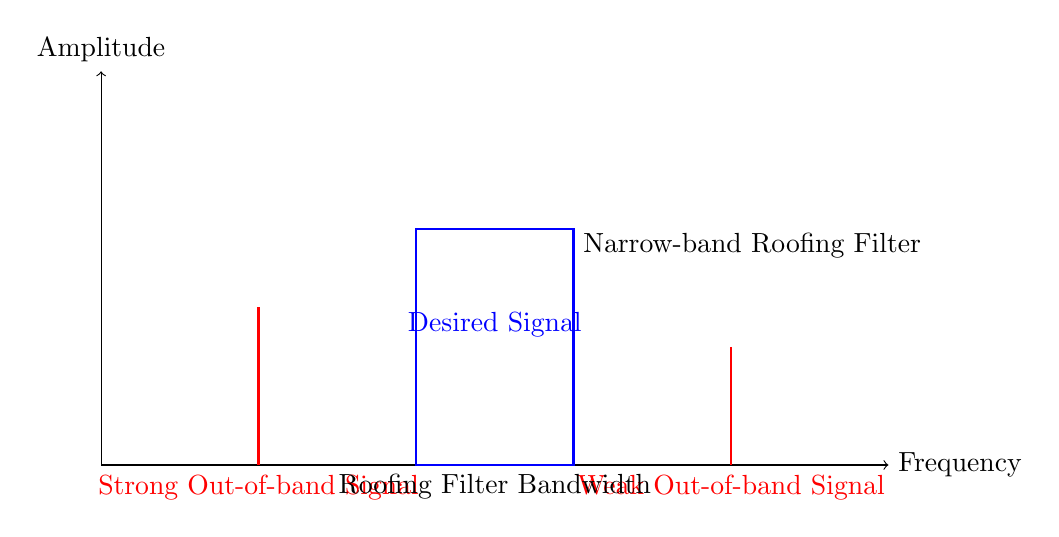
\begin{tikzpicture}
    % Draw axes
    \draw[->] (0,0) -- (10,0) node[right] {Frequency};
    \draw[->] (0,0) -- (0,5) node[above] {Amplitude};

    % Draw a rectangle for the desired frequency range with a narrow-band filter
    \draw[blue, thick] (4,0) rectangle (6,3) node[midway, above] {Desired Signal};
    
    % Draw out-of-band signals
    \draw[red, thick] (2,2) -- (2,0) node[below] {Strong Out-of-band Signal};
    \draw[red, thick] (8,1.5) -- (8,0) node[below] {Weak Out-of-band Signal};

    % Labels
    \node[below] at (5,0) {Roofing Filter Bandwidth};
    \node[above right] at (6,2.5) {Narrow-band Roofing Filter};
\end{tikzpicture}
\end{center}
This diagram represents the frequency spectrum where the narrow-band roofing filter effectively isolates the desired signal while attenuating strong out-of-band signals, thus improving the blocking dynamic range and overall performance of the receiver.
